\documentclass[fleqn,11pt]{article}

\usepackage[letterpaper,margin=0.75in]{geometry}

\usepackage{amsmath}
\usepackage{booktabs}
\usepackage{graphicx}
\usepackage{listings}

\setlength{\parindent}{1.4em}

\begin{document}

\lstset{
  language=Python,
  basicstyle=\small,          % print whole listing small
  keywordstyle=\bfseries,
  identifierstyle=,           % nothing happens
  commentstyle=,              % white comments
  stringstyle=\ttfamily,      % typewriter type for strings
  showstringspaces=false,     % no special string spaces
  numbers=left,
  numberstyle=\tiny,
  numbersep=5pt,
  frame=tb,
}

\title{Reliable Transport (Lab 2) Report}

\author{Luke Dickinson}

\date{2/22/2017}

\maketitle

\section{Introduction}

TCP is one of the core protocols that make the Internet possible. Even through the TCP layer sits on top an unreliable layer, the IP layer, TCP can create a reliable connection between nodes on the Internet. Using Bene with TCP implemented, we are able to run these simulations. We simulate different situations using TCP to see how TCP will function in these cases. We will test networks which drop packets at different rates. We will examine the effects of fast retransmit in TCP. We will also simulate different window sizes to measure the effect it has on throughput and queueing delay. 

\section{Basic Tests}
This section includes a network that consisting of 2 nodes. We set the bandwidth between the nodes to 10 Mbps, and set the propagation delay between the nodes to 10 ms.  We use the TCP protocol to send a file.

 \subsection{First simulation of a two node network}
For the first simulation, we use the network described above and set the window size to 3,000. We set our mss to 1,000. We send a file called "test.txt" of size 10,000 bytes from one node to the other. We test the following loss rates: 0\%, 10\%, 20\%, 50\%.

\subsubsection{First simulation of a two node network: 0\%}
This simulation can be run with the following command: python lab2-basic-1.py -f test.txt -l 0.0\\ \\
The last 10 lines output of this simulation:\\
0.0532 application got 1000 bytes\\
0.0532 n2 (2) sending TCP ACK to 1 for 8000\\
0.054 n2 (2) received TCP segment from 1 for 8000\\
0.054 application got 1000 bytes\\
0.054 n2 (2) sending TCP ACK to 1 for 9000\\
0.0624 n1 (1) sending TCP segment to 2 for 9000\\
0.0732 n2 (2) received TCP segment from 1 for 9000\\
0.0732 application got 1000 bytes\\
0.0732 n2 (2) sending TCP ACK to 1 for 10000\\
Success! both files match\\

When we used a loss rate of 0\%, test.txt was sent in 0.0732 seconds.

\subsubsection{First simulation of a two node network: 10\%}
This can be run with the following command: python lab2-basic-1.py -f test.txt -l 0.10\\ \\
The last 10 lines output of this simulation:\\
0.0532 application got 1000 bytes\\
0.0532 n2 (2) sending TCP ACK to 1 for 8000\\
0.054 n2 (2) received TCP segment from 1 for 8000\\
0.054 application got 1000 bytes\\
0.054 n2 (2) sending TCP ACK to 1 for 9000\\
0.0624 n1 (1) sending TCP segment to 2 for 9000\\
0.0732 n2 (2) received TCP segment from 1 for 9000\\
0.0732 application got 1000 bytes\\
0.0732 n2 (2) sending TCP ACK to 1 for 10000\\
Success! both files match\\

When we used a loss rate of 10\%, test.txt was sent in also 0.0732 seconds. In this case, we didn't lose any packets, even though we had a 10\% chance to lose each packet.

\subsubsection{First simulation of a two node network: 20\%}
This can be run with the following command: python lab2-basic-1.py -f test.txt -l 0.20\\ \\
The last 10 lines output of this simulation:\\
4.094 n2 (2) sending TCP ACK to 1 for 9000\\
4.0948 n2 (2) received TCP segment from 1 for 9000\\
4.0948 application got 1000 bytes\\
4.0948 n2 (2) sending TCP ACK to 1 for 10000\\
5.0832 n1 (1) sending TCP segment to 2 for 9000\\
5.0832 n1 (1) retransmission timer fired\\
5.094 n2 (2) received TCP segment from 1 for 9000\\
5.094 application got 0 bytes\\
5.094 n2 (2) sending TCP ACK to 1 for 10000\\
Success! both files match\\

When we used a loss rate of 20\%, test.txt was sent in 5.094 seconds. We can see multiple packets lost in a row (the ACK for 10,000 and then the packet 9,000) sometimes result in a timeout. These drasticly increase the time needed to send the entire file.

\subsubsection{First simulation of a two node network: 50\%}
This can be run with the following command: python lab2-basic-1.py -f test.txt -l 0.50\\\\
The last 10 lines output of this simulation:\\
21.0732 n2 (2) received TCP segment from 1 for 7000\\
21.0732 application got 0 bytes\\
21.0732 n2 (2) sending TCP ACK to 1 for 9000\\
21.0832 n1 (1) sending TCP segment to 2 for 9000\\
22.0832 n1 (1) sending TCP segment to 2 for 9000\\
22.0832 n1 (1) retransmission timer fired\\
22.094 n2 (2) received TCP segment from 1 for 9000\\
22.094 application got 1000 bytes\\
22.094 n2 (2) sending TCP ACK to 1 for 10000\\
Success! both files match\\

When we used a loss rate of 50\%, test.txt was sent in 22.094 seconds. Similar to the simulation with 20\% loss rate, this simulation has enough loss to result in a timeout. In addition, we can see that packet with sequence 7000 gets through, but the application gains 0 bytes. This is because packet with sequence 7000 had already gone through, but the ACK had been lost. 

 \subsection{Second simulation of a two node network}
For the second simulation, we use the network described above and set the window size to 10,000. We set our mss to 1,000. We send a file called "internet-architecture.pdf" of size 514,520 bytes from one node to the other. We test the following loss rates: 0\%, 50\%.

\subsubsection{Second simulation of a two node network: 0\%}
This can be run with the following command: python lab2-basic-2.py -f internet-architecture.pdf -l 0.0\\\\
The last 10 lines output of this simulation:\\
1.0732 n2 (2) received TCP segment from 1 for 512000\\
1.0732 application got 1000 bytes\\
1.0732 n2 (2) sending TCP ACK to 1 for 513000\\
1.074 n2 (2) received TCP segment from 1 for 513000\\
1.074 application got 1000 bytes\\
1.074 n2 (2) sending TCP ACK to 1 for 514000\\
1.074416 n2 (2) received TCP segment from 1 for 514000\\
1.074416 application got 520 bytes\\
1.074416 n2 (2) sending TCP ACK to 1 for 514520\\
Success! both files match\\

When we used a loss rate of 0\%, internet-architecture.pdf was sent in 1.074416 seconds.

\subsubsection{Second simulation of a two node network: 50\%}
This can be run with the following command: python lab2-basic-2.py -f internet-architecture.pdf -l 0.50\\\\
The last 10 lines output of this simulation:\\
398.1016 n1 (1) sending TCP segment to 2 for 514000\\
398.112016 n2 (2) received TCP segment from 1 for 514000\\
398.112016 application got 520 bytes\\
398.112016 n2 (2) sending TCP ACK to 1 for 514520\\
399.1016 n1 (1) sending TCP segment to 2 for 514000\\
399.1016 n1 (1) retransmission timer fired\\
399.112016 n2 (2) received TCP segment from 1 for 514000\\
399.112016 application got 0 bytes\\
399.112016 n2 (2) sending TCP ACK to 1 for 514520\\
Success! both files match\\

When we used a loss rate of 50\%, internet-architecture.pdf was sent in 399.1120 seconds. This is almost 400 times longer than the simulation with a 0\% loss rate!

\section{Fast Retransmit}
In this section, we want to see the effect TCP's fast retransmit has on total transfer time. We will run a simulation once with fast transmit off, and once with fast transmit on.

We will use the same network as in the basic test section. We use a network that consists of 2 nodes. We set the bandwidth between the nodes to 10 Mbps, and set the propagation delay between the nodes to 10 ms. We set our mss to 1,000. We use the TCP protocol to send the "internet-architecture.pdf" file. We set the loss rate to 20\%.

 \subsection{Fast Retransmit Simulation: Off}
This can be run with the following command: python lab2-fast-1.py -f internet-architecture.pdf -l 0.2\\\\
The last 10 lines output of this simulation:\\
68.978 n2 (2) received TCP segment from 1 for 511000\\
68.978 application got 2000 bytes\\
68.978 n2 (2) sending TCP ACK to 1 for 513000\\
68.9788 n2 (2) received TCP segment from 1 for 513000\\
68.9788 application got 1000 bytes\\
68.9788 n2 (2) sending TCP ACK to 1 for 514000\\
68.979216 n2 (2) received TCP segment from 1 for 514000\\
68.979216 application got 520 bytes\\
68.979216 n2 (2) sending TCP ACK to 1 for 514520\\
Success! both files match\\

With a loss rate of 20\% and without the use fast retransmit, internet-architecture.pdf was sent in 68.979216 seconds.

 \subsection{Fast Retransmit Simulation: On}
This can be run with the following command: python lab2-fast-1.py -f internet-architecture.pdf -l 0.2 -r\\\\
The last 10 lines output of this simulation:\\
34.4084 n2 (2) sending TCP ACK to 1 for 512000\\
34.408816 n2 (2) received TCP segment from 1 for 514000\\
34.408816 application got 0 bytes\\
34.408816 n2 (2) sending TCP ACK to 1 for 512000\\
35.3976 n1 (1) sending TCP segment to 2 for 512000\\
35.3976 n1 (1) retransmission timer fired\\
35.4084 n2 (2) received TCP segment from 1 for 512000\\
35.4084 application got 2520 bytes\\
35.4084 n2 (2) sending TCP ACK to 1 for 514520\\
Success! both files match\\

With a loss rate of 20\%,  and with the use fast retransmit, internet-architecture.pdf was sent in 35.4084 seconds. This is almost twice as fast than the simulation that did not use fast retransmit.

\section{Experiments}
In this section, we explore the effect the size of TCP's window size has on throughput and average queueing delay on file transfer. 

We will use the a similar network as in the previous sections. We use a network that consists of 2 nodes. We set the bandwidth between the nodes to 10 Mbps, and set the propagation delay between the nodes to 10 ms. We set our mss to 1,000. We also set the queue size to 100 packets. We use the TCP protocol to send the "internet-architecture.pdf" file. We set the loss rate to 0\%.

To measure throughput, we take the file size and divide it by the time it takes for the file to completely transfer. We measure the average queueing delay by aggerating the total queueing delay experienced from every packet sent and dividing it by the total number of packets sent. 

We will run our simulation 6 times, with the following windows sizes: 1,000, 2,000, 5,000, 10,000, 15,000, 20,000. It may be helpful to point out that because our mss is 1,000, a window size of 1,000 is a window size of 1 packet. This may be useful in understanding why there is no queueing delay.\\\\
\subsection{Window Size Experiment Commands}
The following commands are executed to run the experiments: \\\\
For a window size of 1,000: python lab2-experiments-1.py -f internet-architecture.pdf\\
For a window size of 2,000: python lab2-experiments-2.py -f internet-architecture.pdf\\
For a window size of 5,000: python lab2-experiments-3.py -f internet-architecture.pdf\\
For a window size of 10,000: python lab2-experiments-4.py -f internet-architecture.pdf\\
For a window size of 15,000: python lab2-experiments-5.py -f internet-architecture.pdf\\
For a window size of 20,000: python lab2-experiments-6.py -f internet-architecture.pdf\\

\subsection{Data of Window Size Experiments}
In the graphs below, we show our experimental data. \\

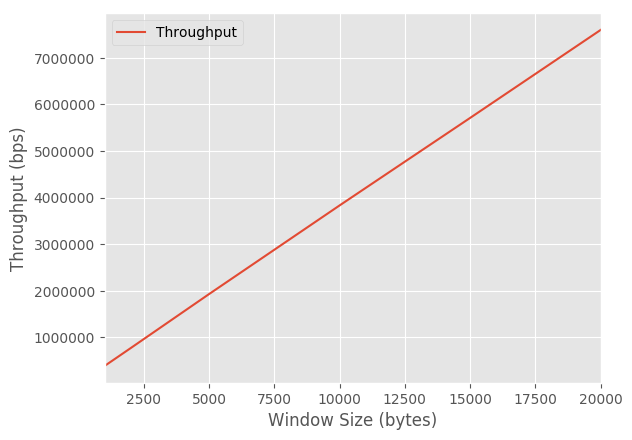
\includegraphics[width=11cm]{lab2-graph1}\\

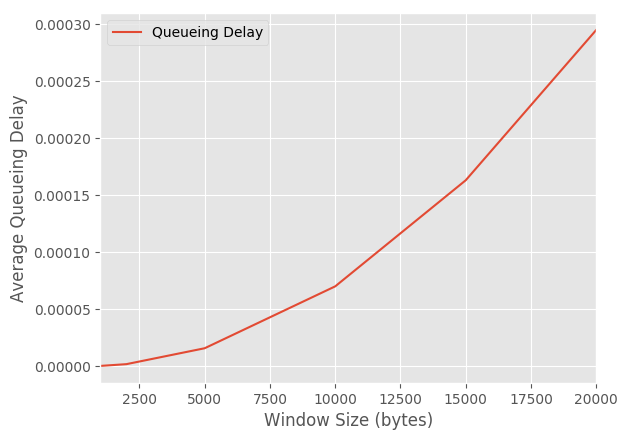
\includegraphics[width=11cm]{lab2-graph2}\\

\subsection{Analysis of Window Size Experiments}
As obviously shown in the first graph, throughput is linearly correlated with window size. The bigger the window size, the faster the file can transfer. Although, we expect this linear correlation is lost when the window size is as big or bigger than the file size. 

Queueing delay seems to have some form of exponential growth. This makes sense, as the more packets we send at once, the longer the packets will have to wait in a queue. This growth is exponential because as more packets are sent, not only are more packets getting stuck in queues, the time spend in a queue grows as the number of packets in front of a packet grows.


\end{document}
